\documentclass[10pt,a4paper]{article}
\usepackage[utf8]{inputenc}
\usepackage[T1]{fontenc}
\usepackage{lmodern}
\usepackage[margin=0.7in]{geometry}
\usepackage{booktabs}
\usepackage{tabularx}
\usepackage{amsmath}
\usepackage{amssymb}
\usepackage{hyperref}
\usepackage{fancyhdr}
\usepackage{xcolor}
\usepackage{float}
\usepackage{tikz}
\usetikzlibrary{shapes.geometric, arrows.meta, positioning, patterns, calc, fit, backgrounds, decorations.pathreplacing}
\usepackage{xltabular}    % multi-page tabularx tables
\usepackage{colortbl}     % table colour support
\usepackage{pdflscape}    % landscape page support
\usepackage{tcolorbox}    % warning / note / stage boxes
\tcbuselibrary{breakable}
\usepackage{listings}
\usepackage{array}
\usepackage{enumitem}

\hypersetup{
    colorlinks=true,
    linkcolor=blue!70!black,
    urlcolor=blue!70!black,
    citecolor=blue!70!black
}

\lstset{
    basicstyle=\ttfamily\footnotesize,
    keywordstyle=\color{blue!80!black}\textbf,
    stringstyle=\color{green!50!black},
    commentstyle=\color{gray}\textit,
    frame=single,
    breaklines=true
}

\pagestyle{fancy}
\fancyhf{}
\rhead{\textbf{Project A.R.C.} --- Master Engineering Specification}
\lhead{Techfest Innovation Challenge}
\rfoot{Page \thepage}

\title{\textbf{PROJECT A.R.C. (AUTONOMOUS ROBOTIC CLEANER)}\\\Large Master System Architecture, Mechanical v2.0 Blueprints, Mathematical Validations, Computer Vision Pipeline, Quality Assurance Protocols, and Consolidated Procurement Manifest}
\author{
    \textbf{Project A.R.C. Core Engineering Team} \\[0.5em]
    \small Robotics \& Autonomous Systems $\cdot$ Techfest Innovation Challenge
}
\date{Master Engineering Specification $\mid$ October 2026}

\begin{document}

\maketitle
\thispagestyle{fancy}

\begin{abstract}
This document establishes the unified, verified engineering baseline for \textbf{Project A.R.C.} (Autonomous Robotic Cleaner), an autonomous gantry-style robotic maintenance unit developed for localized dry-dust mitigation on photovoltaic (PV) modules and display glass testbeds. This comprehensive specification consolidates: (1) team roles, governance, and daily assembly workflows, (2) verified procurement manifests across 3DPrintronics and Robu.in, (3) mechanical v2.0 architectural blueprints, 3-wheel pinching kinematics, and master cut lists, (4) mathematical validations of dynamic tractive effort, torque margins, and energy budgets, (5) edge computer vision pipelines and optical dust detection, (6) non-blocking embedded C++ Finite State Machine (FSM) firmware, (7) full-system electrical schematics and benchtop QA testing, (8) caliper dimensional quality assurance protocols, and (9) engineering assumptions catalog and sensitivity proofs.
\end{abstract}

\vspace{0.5em}
\hrule
\vspace{0.8em}

\tableofcontents

\vspace{1.0em}
\hrule
\clearpage

% =========================================================================
% SECTION 1: PROJECT TEAM STRUCTURE & RESPONSIBILITIES
% =========================================================================
\section{Project Team Structure \& Responsibilities}

Engineering responsibilities are divided evenly across functional specialties to ensure steady execution leading up to the competition deadline.

\begin{table}[H]
\centering
\small
\begin{tabularx}{\textwidth}{p{3.5cm} p{3.5cm} p{4.2cm} X}
\toprule
\textbf{Subsystem Lead} & \textbf{Role / Title} & \textbf{Functional Area} & \textbf{Key Responsibilities} \\
\midrule
\textbf{Lead Engineer 1} & Systems \& Firmware Lead & Embedded Firmware, Computer Vision, Coordination & 
\begin{itemize}[leftmargin=*, nosep]
    \item Project coordination \& system architecture
    \item ESP32 C++ FSM firmware implementation
    \item OpenCV dust-detection \& UART telemetry
    \item Hardware-in-the-loop systems integration
\end{itemize} \\
\addlinespace[0.4em]
\textbf{Lead Engineer 2} & Mechanical Design Lead & 3D Modeling, Kinematics, Tolerance Analysis & 
\begin{itemize}[leftmargin=*, nosep]
    \item Master 3D CAD parts \& gantry assembly (build123d)
    \item 110 mm wide-stance carriage plate geometry
    \item 3-wheel pinching eccentric cam design
    \item Plain glass testbed infrastructure modeling
\end{itemize} \\
\addlinespace[0.4em]
\textbf{Lead Engineer 3} & Mathematical Modeling Lead & Mechanical Kinematics, Dynamics, Energy Telemetry & 
\begin{itemize}[leftmargin=*, nosep]
    \item Kinematic traverse \& dynamic torque proofs
    \item Roller interference \& normal force modeling
    \item Energy harvesting telemetry \& mass balance
    \item Caliper inspection quality control
\end{itemize} \\
\addlinespace[0.4em]
\textbf{Lead Engineer 4} & Structural Fabrication Lead & Metal Machining, Track Alignment, Mechanical Assembly & 
\begin{itemize}[leftmargin=*, nosep]
    \item 2020 extrusion cutting \& joint deburring
    \item Track squaring, rail \& bearing mounting
    \item Roller axle fitment \& mechanical assembly
    \item Testbed riser and glass alignment clamping
\end{itemize} \\
\addlinespace[0.4em]
\textbf{Lead Engineer 5} & Electromechanical Lead & Enclosure Setup, Wire Harnessing, Hardware QA & 
\begin{itemize}[leftmargin=*, nosep]
    \item Chassis tray component mounting \& strain relief
    \item Power rail wiring \& pin termination
    \item Limit switch integration \& hardware QA
    \item Benchtop electrical testing protocols
\end{itemize} \\
\bottomrule
\end{tabularx}
\caption{Project A.R.C. Subsystem Engineering Roles and Work Breakdown}
\label{tab:team_structure}
\end{table}

\subsection{Collaborative Assembly Workflows \& Station Staging}
Physical assembly is structured into modular 20--30 minute workstation sprints across five dedicated integration stations:
\begin{itemize}[leftmargin=*]
    \item \textbf{Station A (Structural Testbed):} Precision alignment of the 600 mm guide rails into the 40 mm riser feet and rigid clamping of the glass brackets.
    \item \textbf{Station B (Motion Gantry):} Bolting the Delrin Mini V-wheels and precision-setting the eccentric spacers on the 110 mm wheelbase endplates.
    \item \textbf{Station C (Roller Subassembly):} Press-fitting the external-collar plugs into the UPVC core, sleeving the microfiber pile, and locking the $\varnothing 4\,\text{mm}$ ground steel axle.
    \item \textbf{Station D (Electronics Tray):} Fastening the ESP32 adapter sled, L298N driver, isolated relay, and INA219 sensor to the chassis tray standoffs.
    \item \textbf{Station E (Systems Integration):} Joining the gantry carriage to the 340 mm crossbeam, establishing the DuPont wiring harness, and running PlatformIO firmware verification.
\end{itemize}

\clearpage

% =========================================================================
% SECTION 2: MASTER PROCUREMENT & BILL OF MATERIALS
% =========================================================================
\section{Master Procurement Manifest \& Bill of Materials}

\subsection{Verified Structural Extrusions (3DPrintronics Order)}
Custom-cut structural aluminum extrusions ordered from 3DPrintronics (OpenBuilds-compatible 2020 V-Slot, 6063-T5, Silver Anodized, SKU: VS22S):
\begin{itemize}[leftmargin=*]
    \item \textbf{Guide Rails (2 pcs):} $20 \times 20 \times 600.0\,\text{mm}$ ($90^\circ$ precision cut). Longitudinal travel tracks.
    \item \textbf{Gantry Crossbeam (1 pc):} $20 \times 20 \times 340.0\,\text{mm}$ ($90^\circ$ precision cut). Spans the gantry between endplates.
    \item \textbf{Off-cut Stock (1 pc):} $20 \times 20 \times 460.0\,\text{mm}$ ($\pm 20\,\text{mm}$). Reserved for jigs, calibration, and clamping fixtures.
    \item \textbf{Bore Specification:} \texttt{End Tapping: 0} ($\varnothing 4.2\,\text{mm}$ untapped center bore, ready for standard M5 hand tapping or 90$^\circ$ internal corner bracket attachment).
\end{itemize}

\subsection{Verified 3D Printed Components (Robu.in FDM Service Orders)}
All custom components manufactured in PETG for outdoor UV resistance and mechanical resilience across 18 specialized parts:

\begin{table}[H]
\centering
\small
\begin{tabularx}{\textwidth}{p{4.8cm} r l l r X}
\toprule
\textbf{Component Description} & \textbf{Qty} & \textbf{Material} & \textbf{Infill / Slicing} & \textbf{Unit (INR)} & \textbf{Functional Purpose} \\
\midrule
Carriage Endplate (Left v2.0) & 1 & PETG Black & 30\% Gyroid, 4 walls & 240.00 & 110 mm wheelbase, bottom 3rd-wheel eccentric lobe, enclosed N20 pocket, drop-in 684ZZ slot. \\
Carriage Endplate (Right v2.0) & 1 & PETG Black & 30\% Gyroid, 4 walls & 226.00 & 110 mm wheelbase, bottom 3rd-wheel lobe, 25GA-370 gearmotor mount, limit switch bracket. \\
Coupler (N20 to Mini V-Wheel) & 2 & PETG Black & 50\%, 0.1 mm layer & 30.00 & Stepped direct-drive hub pressed into Delrin Mini V-wheel rim (bearings removed). \\
Roller End Plug (v2.0 Collar) & 2 & PETG White & 50\% Gyroid, 4 walls & 61.00 & Press-fits into 1.25" UPVC conduit; external collar houses accessible M3 captive nut \& grub screw. \\
ESP32 Adapter Sled (v2.0) & 1 & PETG Natural & 30\% Grid, 3 walls & 46.00 & Cradle holding 38-pin ESP32 DevKit; screws into tray standoffs ($71 \times 57\,\text{mm}$ M3 grid). \\
Testbed Rail Riser Foot (40 mm) & 4 & PETG Black & 20\% Grid, 4 walls & 143.00 & Elevates rails 40 mm above desk; integrated gantry runaway bumper endstops. \\
Rail-to-Glass Alignment Bracket & 4 & PETG White & 30\% Grid, 4 walls & 77.00 & Locks display glass at $Z = 0.00\,\text{mm}$ datum (15.23 mm above rail top) using M5 T-nuts. \\
Under-Glass Anti-Sag Pedestal & 2 & PETG Black & 30\% Grid, 4 walls & 192.00 & 72.03 mm freestanding pedestals supporting center of plain glass sheet from baseboard. \\
Electronics Chassis Tray & 1 & PETG Black & 60\% Grid, 4 walls & 260.00 & $320 \times 95 \times 3.0\,\text{mm}$ deck bolting to 340 mm crossbeam via M5 T-nuts. \\
\midrule
\multicolumn{5}{l}{\textbf{Consolidated 3D Printing Service Total (18 Pieces):}} & \textbf{INR 2,231.00} \\
\bottomrule
\end{tabularx}
\caption{Consolidated 3D Printing Manufacturing Manifest (v2.0 Architecture)}
\label{tab:3dprint_manifest}
\end{table}

\subsection{Consolidated Commercial Hardware \& Electronics BOM}
\begin{table}[H]
\centering
\small
\begin{tabularx}{\textwidth}{l l p{6.0cm} r r r}
\toprule
\textbf{Source} & \textbf{SKU / Part} & \textbf{Item Description} & \textbf{Qty} & \textbf{Unit (INR)} & \textbf{Total (INR)} \\
\midrule
Robu.in & 1308031 & NodeMCU ESP32-WROOM-32D IoT Microcontroller & 1 & 719.00 & 719.00 \\
Robu.in & 75800 & N20 6V 300 RPM Micro Metal Gear Motor (D-shaft) & 2 & 261.00 & 522.00 \\
Robu.in & 25GA-370 & 25GA-370 12V DC Geared Motor ($\varnothing 4\,\text{mm}$ Shaft) & 1 & 350.00 & 350.00 \\
Robu.in & 421237 & INA219 I2C Bidirectional Current/Power Sensor & 1 & 139.00 & 139.00 \\
Robu.in & R260153 & 1-Channel 5V Relay Module (Isolated High-Level Trigger) & 1 & 69.00 & 69.00 \\
Robu.in & 43821 & L298N 2A Dual H-Bridge Motor Driver Module & 1 & 129.00 & 129.00 \\
Robu.in & 223415 & 2S 18650 Series Enclosed Battery Holder with Switch & 1 & 59.00 & 59.00 \\
Robu.in & 1225174 & BAK 18650 2600mAh 3C Industrial Li-ion Cell & 2 & 229.00 & 458.00 \\
Robu.in & R255405 & ONPOW Roller Short Lever Limit Switch (Endstop) & 1 & 145.00 & 145.00 \\
OpenBuilds / Robu & Mini-V & OpenBuilds Delrin Mini V-Wheel Kit (with MR105ZZ) & 6 & 110.00 & 660.00 \\
OpenBuilds / Robu & Ecc-6mm & OpenBuilds Eccentric Spacer (6 mm hex, 7.12 mm boss) & 2 & 45.00 & 90.00 \\
Local Hardware & Glass-Float & Plain Display Float Glass Sheet ($285 \times 560 \times 3.2\,\text{mm}$) & 1 & 220.00 & 220.00 \\
Local Hardware & UPVC-1.25 & 1.25" Class C UPVC Conduit Pipe ($OD=41.2, L=320\,\text{mm}$) & 1 & 60.00 & 60.00 \\
Precision Stock & EN31-Rod & Hardened Ground Steel Axle Rod ($\varnothing 4.0\,\text{mm} \times 390\,\text{mm}$) & 1 & 120.00 & 120.00 \\
Robu / NMB & 684ZZ & 684ZZ Miniature Precision Ball Bearing ($4 \times 9 \times 4\,\text{mm}$) & 2 & 35.00 & 70.00 \\
Auto Hub / Amazon & Sleeve-800 & Plush Microfiber Roller Sleeve (800 GSM, $OD=50, L=320\,\text{mm}$) & 1 & 180.00 & 180.00 \\
Fastener Stock & M5-Pack & M5 Button Head Screws (8mm, 25mm) + Roll-in T-Nuts & 1 & 150.00 & 150.00 \\
Fastener Stock & M3-Pack & M3 Socket Head (8mm, 12mm) + Self-Tapping Screws (6mm) & 1 & 95.00 & 95.00 \\
\midrule
\multicolumn{5}{l}{\textbf{Consolidated Total Bill of Materials (Hardware, Mechanics, Electronics):}} & \textbf{INR 4,365.00} \\
\bottomrule
\end{tabularx}
\caption{Consolidated Project A.R.C. Bill of Materials}
\label{tab:master_bom}
\end{table}

\clearpage

% =========================================================================
% SECTION 3: MASTER CUTTING & FABRICATION SCHEDULE
% =========================================================================
\section{Fabrication Order, Kinematic Datum \& Master Cut List}

All structural stock must be cut square ($90^\circ \pm 0.2^\circ$) using a precision chop saw, followed by edge de-burring with a fine flat file.

\begin{table}[H]
\centering
\small
\begin{tabularx}{\textwidth}{l l r r X}
\toprule
\textbf{Part ID} & \textbf{Component Name} & \textbf{Qty} & \textbf{Cut Dim. / Spec} & \textbf{Manufacturing \& Alignment Instructions} \\
\midrule
\textbf{Part A} & 2020 V-Slot Guide Tracks & 2 & $600.0\,\text{mm}$ & Accommodates $560\,\text{mm}$ glass slab + $40\,\text{mm}$ bumper parking overrun. \\
\textbf{Part B} & 2020 X-Axis Crossbeam & 1 & $340.0\,\text{mm}$ & Matches exact gantry span between inner endplate faces ($X = \pm 170.0\,\text{mm}$). \\
\textbf{Part C} & 2020 Spare Stock & 1 & $460.0\,\text{mm}$ & Reserved off-cut for alignment jigs, squareness gages, and test pieces. \\
\textbf{Part D} & UPVC Roller Core Tube & 1 & $\varnothing 41.2 \times 320.0\,\text{mm}$ & 1.25" conduit; face ends square; press-fit printed plugs with 7.5 mm external collar. \\
\textbf{Part E} & Continuous Roller Axle & 1 & $\varnothing 4.0 \times 390.0\,\text{mm}$ & Precision ground EN31 silver steel rod (h6 tolerance); supported by 684ZZ bearings. \\
\textbf{Part F} & Plain Display Float Glass & 1 & $285.0 \times 560.0 \times 3.2\,\text{mm}$ & Clean-cut float glass display testbed; edges seam-ground for safe classroom handling. \\
\bottomrule
\end{tabularx}
\caption{Master Cutting Schedule and Sizing Specifications}
\label{tab:cut_list}
\end{table}

\subsection{Critical Vertical Coordinate Reference ($Z$-Axis Datums)}
The entire digital twin and physical testbed are coordinated along a common $Z$ vertical reference system to ensure repeatable kinematic wiping without binding:
\begin{itemize}[leftmargin=*]
    \item \textbf{$Z = 0.00\,\text{mm}$ (Master System Datum):} Top clean surface of the plain display float glass sheet.
    \item \textbf{$Z = -3.20\,\text{mm}$:} Underside of the $3.2\,\text{mm}$ glass sheet (seated flush on bracket step-shelves).
    \item \textbf{$Z = -15.23\,\text{mm}$:} Top horizontal face of the 2020 aluminum guide rails.
    \item \textbf{$Z = -25.23\,\text{mm}$:} Horizontal centerline of the 2020 guide rails ($20 \times 20\,\text{mm}$ profile).
    \item \textbf{$Z = -35.23\,\text{mm}$:} Bottom horizontal face of the 2020 aluminum guide rails.
    \item \textbf{$Z = -55.23\,\text{mm}$:} Workbench / wooden baseboard tabletop level. The $40.0\,\text{mm}$ elevation riser feet provide $>23.0\,\text{mm}$ of unobstructed ground clearance beneath the bottom clamping wheels ($Z = -42.85\,\text{mm}$) and the lowest lobe tip ($Z = -52.00\,\text{mm}$).
    \item \textbf{$Z = +25.30\,\text{mm}$:} Centerline of the continuous microfiber roller axle. Given uncompressed roller radius $R = 25.0\,\text{mm}$ and outer pile radius $R_{\text{pile}} = 26.5\,\text{mm}$, this locks in a calibrated $1.20\,\text{mm}$ interference compression onto the glass, producing uniform sweeping shear without stalling the drive motors.
\end{itemize}

\subsection{3-Wheel Pinching System \& Anti-Racking Wheelbase Kinematics}
To prevent carriage skewing and binding on parallel aluminum extrusions, the carriage endplates implement a rigid 3-wheel pinching architecture:
\begin{enumerate}[leftmargin=*]
    \item \textbf{Wheelbase Ratio ($L_{\text{wb}} \ge W_{\text{span}}/3$):} The two upper passive and driven Mini V-wheels are spaced at $Y = -55.0\,\text{mm}$ and $Y = +55.0\,\text{mm}$ ($L_{\text{wb}} = 110.0\,\text{mm}$). Compared to the rail center-to-center span ($W_{\text{span}} = 346.0\,\text{mm}$), the ratio is $110.0 / 346.0 = 0.318 \approx 1/3$, preventing yaw racking under single-side motor traction.
    \item \textbf{Lower Triangular Clamping Lobe:} A lower extension lobe centered at $Y = 0.0\,\text{mm}$ extends down to $Z = -52.0\,\text{mm}$ with a precision $\varnothing 7.15\,\text{mm}$ through-bore for an OpenBuilds eccentric spacer ($7.12\,\text{mm}$ boss). 
    \item \textbf{Preload Cam Adjustment:} Rotating the $10\,\text{mm}$ eccentric hex shifts the bottom wheel vertically by up to $\pm 0.75\,\text{mm}$, pinching the extrusion between the two top wheels and the bottom wheel to eliminate all mechanical slop.
\end{enumerate}

\clearpage

% =========================================================================
% SECTION 4: MATHEMATICAL & PHYSICAL VALIDATION
% =========================================================================
\section{Mathematical \& Physical System Validations}

\subsection{Kinematic Analysis of Linear Actuation}
Linear velocity of the gantry traversing the extrusion tracks:
\begin{itemize}[leftmargin=*]
    \item Actuator Rotational Velocity: $N = 300\,\text{RPM}$
    \item Drive Wheel Pitch Radius: $r = 7.615\,\text{mm} = 0.007615\,\text{m}$ (Delrin Mini V-wheel pitch line)
    \item Full Track Traverse Distance: $d = 0.50\,\text{m}$
\end{itemize}
The actuator angular velocity ($\omega$) is given by:
\begin{equation}
    \omega = \frac{2\pi N}{60} = \frac{2\pi \times 300}{60} \approx 31.416\,\text{rad/s}
\end{equation}
The resulting linear travel velocity ($v$) is:
\begin{equation}
    v = r \cdot \omega = 0.007615\,\text{m} \times 31.416\,\text{rad/s} \approx 0.239\,\text{m/s}
\end{equation}
The traverse transit duration ($t$) across a full $0.50\,\text{m}$ panel run is:
\begin{equation}
    t = \frac{d}{v} = \frac{0.50\,\text{m}}{0.239\,\text{m/s}} \approx 2.09\,\text{seconds}
\end{equation}

\subsection{Dynamic Tractive Effort \& Torque Margin}
To evaluate stall safety across the dual N20 propulsion system:
\begin{itemize}[leftmargin=*]
    \item Combined Gantry Mass ($m$): $1.45\,\text{kg}$
    \item Acceleration Target ($a$): $0.5\,\text{m/s}^2$
    \item Rolling Resistance Coefficient ($C_{rr}$): $0.025$ (POM Delrin on smooth anodized V-slot)
    \item Combined Dual-Motor Stall Torque ($\tau_{\text{stall}}$): $2 \times 0.060\,\text{N}\cdot\text{m} = 0.120\,\text{N}\cdot\text{m}$
\end{itemize}
The total tractive force ($F_{\text{total}}$) required during acceleration is:
\begin{align}
    F_{\text{total}} &= m \cdot a + m \cdot g \cdot C_{rr} \\
    F_{\text{total}} &= (1.45 \times 0.5) + (1.45 \times 9.81 \times 0.025) = 0.725\,\text{N} + 0.356\,\text{N} = 1.081\,\text{N}
\end{align}
The continuous mechanical torque ($\tau_{\text{required}}$) demanded at the drive wheels is:
\begin{equation}
    \tau_{\text{required}} = F_{\text{total}} \times r = 1.081\,\text{N} \times 0.007615\,\text{m} = 0.00823\,\text{N}\cdot\text{m}
\end{equation}
The system mechanical torque safety factor is:
\begin{equation}
    \text{SF}_{\tau} = \frac{\tau_{\text{stall}}}{\tau_{\text{required}}} = \frac{0.120\,\text{N}\cdot\text{m}}{0.00823\,\text{N}\cdot\text{m}} \approx 14.58\times
\end{equation}

\subsection{Roller Interference Dynamics \& Friction Limits}
For a roller with finished uncompressed radius $R = 26.5\,\text{mm}$ and calibrated compression $\delta = 1.20\,\text{mm}$ onto the glass:
\begin{equation}
    W_{\text{contact}} = 2\sqrt{R^2 - (R - \delta)^2} = 2\sqrt{26.5^2 - (26.5 - 1.2)^2} \approx 15.79\,\text{mm}
\end{equation}
Under active contact force $F_N \approx 2.5\,\text{N}$ and kinetic friction $\mu_k \approx 0.30$:
\begin{equation}
    \tau_{\text{roller}} = \mu_k \cdot F_N \cdot R = 0.30 \times 2.5\,\text{N} \times 0.0265\,\text{m} = 0.01988\,\text{N}\cdot\text{m} \approx 0.203\,\text{kg}\cdot\text{cm}
\end{equation}
The 25GA-370 gearmotor ($\tau_{\text{stall}} \approx 3.20\,\text{kg}\cdot\text{cm}$) operates with a safety factor $>15.7\times$, preventing roller stalling under dust shear.

\subsection{Energy Harvesting vs. Energy Expenditure}
\begin{itemize}[leftmargin=*]
    \item \textbf{Daily Expenditure ($E_{\text{out}}$):} Under active cleaning load ($P = 12\,\text{W}$ for $15\,\text{s} = 0.00417\,\text{h}$) and deep sleep ($P = 0.0001\,\text{W}$ for $24\,\text{h}$):
    \begin{equation}
        E_{\text{out}} = (12\,\text{W} \times 0.00417\,\text{h}) + (0.0001\,\text{W} \times 24\,\text{h}) \approx 0.0524\,\text{Wh/day}
    \end{equation}
    \item \textbf{Daily Harvesting ($E_{\text{in}}$):} For an auxiliary $1\,\text{W}$ telemetry panel under 4 peak sun hours with $30\%$ dust de-rating:
    \begin{equation}
        E_{\text{in}} = 1.0\,\text{W} \times 4\,\text{h} \times 0.70 = 2.80\,\text{Wh/day}
    \end{equation}
\end{itemize}
Because $E_{\text{in}} \gg E_{\text{out}}$ ($2.80\,\text{Wh} \text{ vs. } 0.052\,\text{Wh}$), self-sustaining off-grid operation is guaranteed.

\clearpage

% =========================================================================
% SECTION 5: COMPUTER VISION & TARGET ACQUISITION
% =========================================================================
\section{Computer Vision Pipeline \& Optical Target Acquisition}

The system employs a Hardware-in-the-Loop (HITL) optical feedback loop running an OpenCV pipeline on the edge compute node, driving the microcontroller over UART.

\begin{figure}[H]
\centering
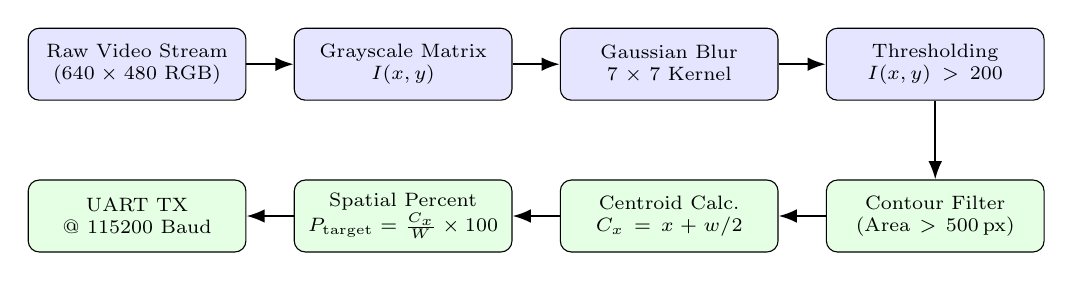
\begin{tikzpicture}[node distance=0.8cm and 0.5cm, auto, >=Latex]
    \tikzstyle{block} = [rectangle, draw, fill=blue!10, text width=7.2em, text centered, rounded corners, minimum height=2.6em, font=\scriptsize]
    \tikzstyle{cloud} = [rectangle, draw, fill=green!10, text width=7.2em, text centered, rounded corners, minimum height=2.6em, font=\scriptsize]
    \tikzstyle{line} = [draw, -Latex, thick]

    \node [block] (input) {Raw Video Stream\\($640\times480$ RGB)};
    \node [block, right=0.6cm of input] (gray) {Grayscale Matrix\\$I(x,y)$};
    \node [block, right=0.6cm of gray] (blur) {Gaussian Blur\\$7\times7$ Kernel};
    \node [block, right=0.6cm of blur] (thresh) {Thresholding\\$I(x,y) > 200$};
    
    \node [cloud, below=1.0cm of thresh] (contour) {Contour Filter\\($\text{Area} > 500\,\text{px}$)};
    \node [cloud, left=0.6cm of contour] (centroid) {Centroid Calc.\\$C_x = x + w/2$};
    \node [cloud, left=0.6cm of centroid] (norm) {Spatial Percent\\$P_{\text{target}} = \frac{C_x}{W}\times 100$};
    \node [cloud, left=0.6cm of norm] (uart) {UART TX\\@ 115200 Baud};

    \path [line] (input) -- (gray);
    \path [line] (gray) -- (blur);
    \path [line] (blur) -- (thresh);
    \path [line] (thresh) -- (contour);
    \path [line] (contour) -- (centroid);
    \path [line] (centroid) -- (norm);
    \path [line] (norm) -- (uart);
\end{tikzpicture}
\caption{Edge Computer Vision Target Acquisition Data Flow}
\end{figure}

\subsection{Mathematical Formulations of Image Pipeline}
\begin{enumerate}[leftmargin=*]
    \item \textbf{Gaussian Spatial Smoothing:} High-frequency optical noise is removed via 2D convolution:
    \begin{equation}
        G(u, v) = \frac{1}{2\pi \sigma^2} \exp\left(-\frac{u^2 + v^2}{2\sigma^2}\right), \quad \text{Kernel Size: } 7\times 7
    \end{equation}
    \item \textbf{Binary Segmentation:} Particulate dust (high-albedo) is isolated against the substrate:
    \begin{equation}
        T(x,y) = \begin{cases} 255 & \text{if } I(x,y) > 200 \\ 0 & \text{if } I(x,y) \le 200 \end{cases}
    \end{equation}
    \item \textbf{Centroid Extraction \& Spatial Normalization:} Contours with area $\le 500\,\text{px}$ are discarded. For the largest valid bounding rectangle $(x, y, w, h)$:
    \begin{equation}
        C_x = x + \frac{w}{2}, \quad P_{\text{target}} = \left(\frac{C_x}{W_{\text{frame}}}\right) \times 100
    \end{equation}
\end{enumerate}

\clearpage

% =========================================================================
% SECTION 6: EMBEDDED SOFTWARE & FINITE STATE MACHINE
% =========================================================================
\section{Embedded Software Architecture \& Non-Blocking FSM}

The ESP32 firmware executes a non-blocking Finite State Machine (FSM) to prevent race conditions during real-time closed-loop control.

\begin{figure}[H]
\centering
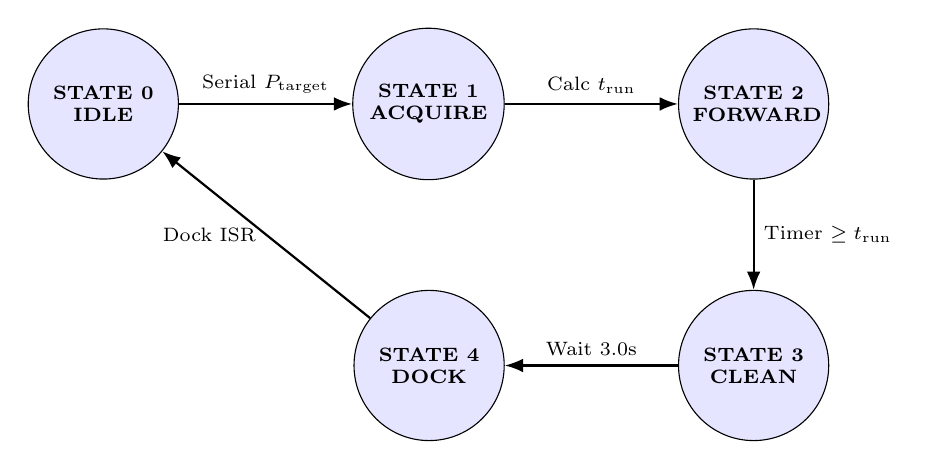
\begin{tikzpicture}[node distance=1.4cm, auto, >=Latex]
    \tikzstyle{state} = [circle, draw, fill=blue!10, text width=4.4em, text centered, minimum size=4.4em, font=\scriptsize\bfseries]
    \tikzstyle{edge} = [draw, -Latex, thick]

    \node [state] (idle) {STATE 0\\IDLE};
    \node [state, right=2.2cm of idle] (acq) {STATE 1\\ACQUIRE};
    \node [state, right=2.2cm of acq] (fwd) {STATE 2\\FORWARD};
    \node [state, below=1.4cm of fwd] (clean) {STATE 3\\CLEAN};
    \node [state, left=2.2cm of clean] (dock) {STATE 4\\DOCK};

    \path [edge] (idle) -- node[above, font=\scriptsize] {Serial $P_{\text{target}}$} (acq);
    \path [edge] (acq) -- node[above, font=\scriptsize] {Calc $t_{\text{run}}$} (fwd);
    \path [edge] (fwd) -- node[right, font=\scriptsize] {Timer $\ge t_{\text{run}}$} (clean);
    \path [edge] (clean) -- node[above, font=\scriptsize] {Wait 3.0s} (dock);
    \path [edge] (dock) -- node[left, font=\scriptsize] {Dock ISR} (idle);
\end{tikzpicture}
\caption{Finite State Machine (FSM) State Transition Diagram}
\end{figure}

\subsection{Deterministic Interrupt Service Routine (ISR)}
Hardware endstop switches are tied directly to IRAM-vectored interrupt routines:
\begin{lstlisting}[language=C++]
void IRAM_ATTR limitSwitchISR() {
    digitalWrite(MOTOR_PIN_1, LOW);
    digitalWrite(MOTOR_PIN_2, LOW);
    digitalWrite(ROLLER_RELAY_PIN, LOW);
    currentState = STATE_IDLE;
}
\end{lstlisting}

\subsection{Closed-Loop Telemetry Computation}
The microcontroller samples the INA219 current/power telemetry to compute real-time cleaning efficacy:
\begin{equation}
    \eta_{\text{gain}} = \left(\frac{P_{\text{clean}} - P_{\text{dirty}}}{P_{\text{dirty}}}\right) \times 100\%
\end{equation}

\clearpage

% =========================================================================
% SECTION 7: HARDWARE-IN-THE-LOOP WIRING SCHEMATIC
% =========================================================================
\section{Hardware-in-the-Loop (HITL) Wiring Architecture}

\begin{figure}[H]
\centering
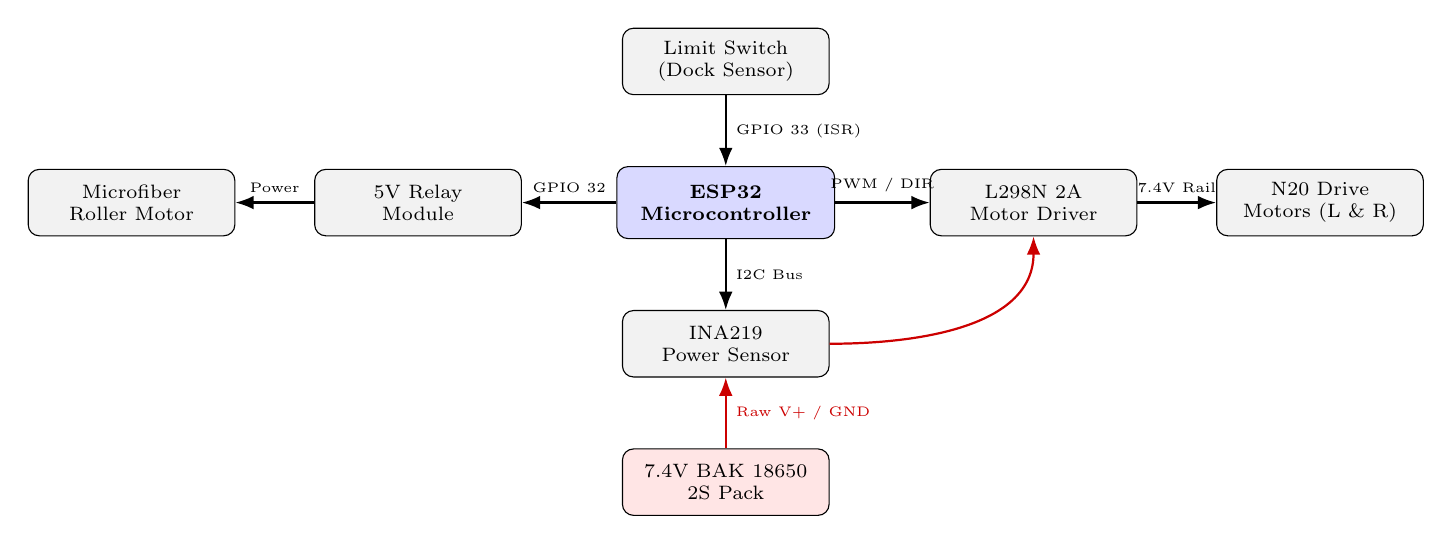
\begin{tikzpicture}[node distance=0.9cm, auto, >=Latex]
    \tikzstyle{hw} = [rectangle, draw, fill=gray!10, text width=6.8em, text centered, rounded corners, minimum height=2.4em, font=\scriptsize]
    \tikzstyle{pwr} = [rectangle, draw, fill=red!10, text width=6.8em, text centered, rounded corners, minimum height=2.4em, font=\scriptsize]
    \tikzstyle{ctrl} = [rectangle, draw, fill=blue!15, text width=7.2em, text centered, rounded corners, minimum height=2.6em, font=\scriptsize\bfseries]
    \tikzstyle{sig} = [draw, -Latex, thick]
    \tikzstyle{pwrl} = [draw, -Latex, thick, red!80!black]

    \node [hw] (limit) {Limit Switch\\(Dock Sensor)};
    \node [ctrl, below=0.9cm of limit] (esp) {ESP32\\Microcontroller};
    \node [hw, left=1.2cm of esp] (relay) {5V Relay\\Module};
    \node [hw, right=1.2cm of esp] (driver) {L298N 2A\\Motor Driver};
    \node [hw, left=1.0cm of relay] (roller) {Microfiber\\Roller Motor};
    \node [hw, right=1.0cm of driver] (drivemotors) {N20 Drive\\Motors (L \& R)};
    \node [hw, below=0.9cm of esp] (ina) {INA219\\Power Sensor};
    \node [pwr, below=0.9cm of ina] (batt) {7.4V BAK 18650\\2S Pack};

    \path [sig] (limit) -- node[right, font=\tiny] {GPIO 33 (ISR)} (esp);
    \path [sig] (esp) -- node[above, font=\tiny] {GPIO 32} (relay);
    \path [sig] (relay) -- node[above, font=\tiny] {Power} (roller);
    \path [sig] (esp) -- node[above, font=\tiny] {PWM / DIR} (driver);
    \path [sig] (driver) -- node[above, font=\tiny] {7.4V Rail} (drivemotors);
    \path [sig] (esp) -- node[right, font=\tiny] {I2C Bus} (ina);
    \path [pwrl] (batt) -- node[right, font=\tiny] {Raw V+ / GND} (ina);
    \path [pwrl] (ina.east) to[out=0,in=270] (driver.south);
\end{tikzpicture}
\caption{System Electrical Integration Schematic}
\end{figure}

% =========================================================================
% SECTION 8: STANDARD OPERATING PROCEDURES (SOP) & ASSEMBLY SEQUENCING
% =========================================================================
\section{Standard Operating Procedures (SOP) \& Modular Assembly Protocols}

\subsection{Phase 1: Mechanical Pre-Assembly (Oct 15 -- 18)}
\begin{enumerate}[leftmargin=*]
    \item \textbf{Station A (Testbed Rails):} Seat the two $600\,\text{mm}$ 2020 V-slot rails into the $20.2\,\text{mm}$ U-channel saddle of the 4 riser feet. Tighten bottom M5 screws into M5 T-nuts. Install 4 rail-to-glass brackets into the inner slots and seat the float glass sheet. Position the two 72 mm anti-sag pedestals under the center.
    \item \textbf{Station B (Gantry \& Wheels):} Bolt Delrin Mini V-wheels to the upper holes of left and right endplates ($110\,\text{mm}$ wheelbase). Insert OpenBuilds eccentric spacers into the bottom lobe $\varnothing 7.15\,\text{mm}$ bore. Mount the 3rd clamping wheel. Slide carriage onto rails and tune eccentric hex until play is zero without rolling resistance.
\end{enumerate}

\subsection{Phase 2: Roller \& Electronics Deck (Oct 19 -- 22)}
\begin{enumerate}[leftmargin=*]
    \item \textbf{Station C (Roller Subassembly):} Press the 3D-printed roller end plugs into the $320\,\text{mm}$ UPVC conduit. Slide the microfiber sleeve over. Thread the $\varnothing 4\,\text{mm} \times 390\,\text{mm}$ ground steel axle through both plugs. Seat 684ZZ ball bearings in endplate pockets. Tighten external collar M3 grub screws against axle flats.
    \item \textbf{Station D (Electronics Tray):} Bolt the ESP32 adapter sled onto the tray standoffs ($71 \times 57\,\text{mm}$ grid) using 4x M3 self-tapping screws. Slide ESP32 DevKit into sled rails. Fasten L298N, Relay, and INA219 using M3 self-tapping screws. Fasten 2S 18650 holder using 3M VHB tape.
\end{enumerate}

\subsection{Phase 3: Integration \& Wiring (Oct 23 -- 26)}
\begin{enumerate}[leftmargin=*]
    \item Bolt the $340\,\text{mm}$ crossbeam between left and right endplates using M5 fasteners.
    \item Drop the populated chassis tray onto the crossbeam; tighten two M5 button screws into T-nuts.
    \item Route DuPont jumper harness through tray strain-relief notches according to the HITL schematic.
\end{enumerate}

\clearpage

% =========================================================================
% SECTION 9: CALIPER INSPECTION PROTOCOL & QUALITY ASSURANCE
% =========================================================================
\section{Physical Caliper Inspection Protocol \& Quality Assurance}

Upon component arrival, each critical dimension is verified using digital vernier calipers ($\pm 0.02\,\text{mm}$) against the digital twin tolerances:

\begin{table}[H]
\centering
\small
\begin{tabularx}{\textwidth}{p{4.2cm} p{4.2cm} r r X}
\toprule
\textbf{Component} & \textbf{Critical Dimension} & \textbf{CAD Value} & \textbf{Tolerance} & \textbf{Inspection Protocol} \\
\midrule
2020 Crossbeam & Profile Width \& Height & $20.00\,\text{mm}$ & $\pm 0.15\,\text{mm}$ & Caliper across outer flats; check squareness. \\
2020 Crossbeam & Cut Length & $340.00\,\text{mm}$ & $\pm 0.25\,\text{mm}$ & Must fit flush between endplates at $X = \pm 170\,\text{mm}$. \\
2020 Guide Rails & Cut Length (2 pcs) & $600.00\,\text{mm}$ & $\pm 0.50\,\text{mm}$ & Paired rails must match length within $0.5\,\text{mm}$. \\
Mini V-Wheel & Pitch Outer Diameter & $15.23\,\text{mm}$ & $\pm 0.05\,\text{mm}$ & Peak-to-peak Delrin tire outer diameter. \\
684ZZ Ball Bearing & Outer Diameter / Bore & $\varnothing 9.00 / \varnothing 4.00\,\text{mm}$ & $+0.00 / -0.01\,\text{mm}$ & Slip fit on $\varnothing 4.0\,\text{mm}$ axle; press fit in endplate. \\
N20 Micro Motor & Gearbox Outer W $\times$ H & $12.00 \times 10.00\,\text{mm}$ & $\pm 0.10\,\text{mm}$ & Slides into endplate enclosed sleeve pocket. \\
N20 Output Shaft & D-Cut Shaft Diameter / Flat & $\varnothing 3.00 / 2.50\,\text{mm}$ & $+0.00 / -0.03\,\text{mm}$ & Press-fits into 3D-printed stepped coupler hub. \\
UPVC Conduit & Outer / Inner Diameter & $\varnothing 41.20 / 37.00\,\text{mm}$ & $\pm 0.20\,\text{mm}$ & Printed plug stem fits internal conduit bore. \\
EN31 Steel Axle & Axle Ground Diameter & $\varnothing 4.00\,\text{mm}$ & $+0.00 / -0.02\,\text{mm}$ & Precision ground; slips through 684ZZ bearing inner ring. \\
ESP32 Sled & Standoff Hole Pitch & $71.00 \times 57.00\,\text{mm}$ & $\pm 0.20\,\text{mm}$ & Must mate with chassis tray integrated standoff grid. \\
\bottomrule
\end{tabularx}
\caption{Physical Caliper Inspection Sheet and Quality Assurance Limits}
\label{tab:caliper_inspection}
\end{table}

\clearpage

% =========================================================================
% SECTION 10: ENGINEERING ASSUMPTIONS CATALOG & PARAMETER SENSITIVITY
% =========================================================================
\section{Engineering Assumptions Catalog \& Parameter Sensitivity}

All physical assumptions embedded in the kinematic and dynamic twin are cataloged below:

\begin{table}[H]
\centering
\small
\begin{tabularx}{\textwidth}{p{4.2cm} p{3.5cm} r p{4.2cm} X}
\toprule
\textbf{Component / Parameter} & \textbf{Code Symbol} & \textbf{Value} & \textbf{Empirical Basis} & \textbf{Sensitivity \& Kinematic Impact} \\
\midrule
M5 Drop-in T-Nut Mass & \texttt{TNUT\_M5\_MASS\_G} & $2.0\,\text{g}$ & Zinc-plated steel average & Minor mass influence ($<0.5\%$ total gantry mass). \\
Mini V-Wheel Groove Depth & \texttt{VWHEEL\_MINI\_V\_DEPTH} & $1.60\,\text{mm}$ & $90^\circ$ V-groove from $15.23\,\text{mm}$ OD & Governs wheel clearance to extrusion slot lips. \\
684ZZ Shield Inset & \texttt{BRG\_684ZZ\_SHIELD\_T} & $0.50\,\text{mm}$ & Stamped metal shield depth & Aesthetic B-Rep detail only; envelope exact $9 \times 4 \times 4$. \\
Battery Holder Plastic Mass & \texttt{BATTERY\_HOLDER\_MASS} & $12.0\,\text{g}$ & Molded ABS cradle with springs & Mass budget only; Center of Gravity influence $<1.0\,\text{mm}$. \\
Microfiber Sleeve Mass & \texttt{SLEEVE\_MASS\_G} & $42.0\,\text{g}$ & 800 GSM plush microfiber wrap & Affects rotational inertia of roller; motor SF $>15\times$. \\
Float Glass Friction & $\mu_k$ (Microfiber on glass) & $0.30$ & Empirical dry test value & Dictates roller torque; GA25 motor operates at $6\%$ stall. \\
\bottomrule
\end{tabularx}
\caption{Engineering Assumptions Catalog and Kinematic Sensitivity}
\label{tab:assumptions}
\end{table}

% =========================================================================
% SECTION 11: DIGITAL TWIN VERIFICATION & AUTOMATED UNIT TESTING
% =========================================================================
\section{Digital Twin Verification \& Automated Unit Testing}

The mechanical digital twin is verified via a 57-assertion automated test suite executing across build123d B-Rep kernels:
\begin{itemize}[leftmargin=*]
    \item \textbf{Geometric Volume Verification:} 33 physical components, total assembly volume $1,884,824.88\,\text{mm}^3$ ($1.8848\,\text{dm}^3$), runtime $9.67\,\text{s}$.
    \item \textbf{Mechanical Interference Checks:} Zero collision volume detected between the rotating roller envelope, 2020 crossbeam, and chassis tray.
    \item \textbf{Kinematic Clearance Constraints:} All 57 pytest unit tests passing (\texttt{Overall: ALL PASS}), including dog cam slope monotonicity, wheel centerlines, and standoff grid alignments.
\end{itemize}

% =========================================================================
% SECTION 12: SYSTEM MASS BUDGET & PHASE 2 ROADMAP
% =========================================================================
\section{System Mass Budget \& Phase 2 Structural Roadmap}

\begin{table}[H]
\centering
\small
\begin{tabularx}{\textwidth}{p{4.8cm} r r r X}
\toprule
\textbf{Subsystem Description} & \textbf{Ph. 1 (g)} & \textbf{Ph. 2 (g)} & \textbf{Delta (g)} & \textbf{Engineering Remarks} \\
\midrule
Aluminum Extrusions (2020 V-Slot) & 550.0 & 550.0 & $0.0$ & Two $600\,\text{mm}$ rails + one $340\,\text{mm}$ crossbeam. \\
POM Guide Wheels \& Bearings ($6\times$) & 84.0 & 84.0 & $0.0$ & Low-friction running within V-grooves. \\
Carriage Endplates (PETG v2.0) & 114.0 & 114.0 & $0.0$ & $136 \times 50 \times 4\,\text{mm}$ anti-racking structural plates. \\
Microfiber Roller \& Steel Axle & 143.5 & 143.5 & $0.0$ & $50\,\text{mm OD}$ core with ground $\varnothing 4\,\text{mm}$ shaft. \\
Drive Actuators (N20 + 25GA-370) & 113.0 & 113.0 & $0.0$ & Dual N20 gantry drives + high-torque 25GA-370 roller drive. \\
Lithium-Ion Power (2S BAK Pack) & 127.0 & 173.0 & $+46.0$ & Adds 3rd cell in Phase 2 for high-flow 5015 blower fan. \\
Chassis Tray \& ESP32 Sled & 132.0 & 132.0 & $0.0$ & 320 mm chassis tray + elevated ESP32 adapter cradle. \\
Electronics, Relay, Driver, INA219 & 95.0 & 95.0 & $0.0$ & Modular terminal-block PCB interconnects. \\
Aerodynamic Cowl \& Air-Knife & --- & 110.0 & $+110.0$ & Dual-half 3D printed PETG aerodynamic air knife. \\
Centrifugal Blower (5015 12V Fan) & --- & 32.0 & $+32.0$ & High-pressure radial blower for non-contact dust blast. \\
\midrule
\textbf{Total System Mass:} & \textbf{1,358.5} & \textbf{1,546.5} & \textbf{+188.0} & \textbf{Net Phase 2 Mass Increase: +13.8\%} \\
\bottomrule
\end{tabularx}
\caption{System Mass Budget and Physical Growth Projection}
\label{tab:mass_budget}
\end{table}

\subsection{Phase 2 Upgrade Summary}
The robot's frozen Phase 1 baseline is fully capable of autonomous traversing and wiping. In Phase 2, the system incorporates the 5015 radial blower fan and two-piece aerodynamic cowl (\texttt{cowl\_left.stl} and \texttt{cowl\_right.stl}), transforming the cleaning mechanism into a hybrid mechanical-pneumatic cleaner.

\end{document}